\documentclass[12pt,letterpaper]{report}
\usepackage[spanish]{babel}
\usepackage[utf8]{inputenc}
\usepackage{graphicx}
\usepackage{adjustbox}


\begin{document}
\setcounter{chapter}{2}
\setcounter{section}{1}
\section{Algoritmos genéticos.}\label{cap.algoritmos_geneticos}

\subsection{Evolución de las especies.}
La evolución no es un evento observable, sino un evento inferido. dado al corto tiempo que dedicamos a observar la naturaleza en comparación al tiempo de existencia de la naturaleza. Es difícil tener pruebas irrefutables de cuánto tiempo ha existido la vida en la Tierra. Sin embargo, dado que es imposible Generación espontánea, la inferencia indica que los seres vivos deben tener su propio origen en el pasado de la misma manera que el presente: de otra criatura, y dada la evidencia de la existencia de restos de algunos de estos organismos ,la falta de existencia de restos antiguos de muchas criaturas actuales, se puede deducir que en el pasado, la existencia de una especie producía la existencia de otra especie, de esta manera para cada generación de especies.
%referenciar 11094-20180116

\begin{figure}[!htb]
	\centering
	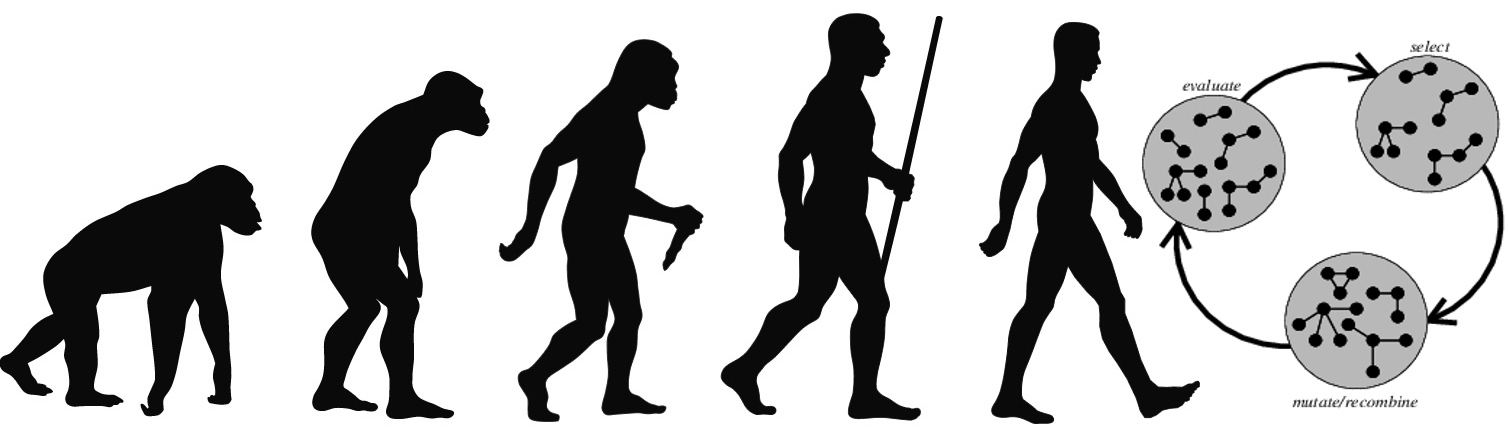
\includegraphics[width=\textwidth]{Img_C2_2.2/evolution.jpg} 
	\caption{Representación de la evolución humana.}
	\label{fig:evolucion}
\end{figure}



Es de esta teoria de donde surgen los algoritmos evolutivos.

\subsubsection{Algoritmos evolutivos}

Los algoritmos evolutivos son metodos de optimizacion y busqueda para dar soluciones a problemas los cuales funcionan bajo la logica de la evolucion de sistemas biologicos.

La idea básica de estos algoritmos es mantener un conjunto de individuos que representan posibles soluciones a un problema. Estos individuos se mezclan y compiten entre sí, siguiendo los principios de la selección natural, y solo los más adaptados sobreviven en el tiempo. Esto conduce a un desarrollo hacia soluciones cada vez más adecuadas.
Los algoritmos evolutivos son una serie de métodos de optimización, Por lo tanto, intentan encontrar una tupla de valores (xi,...,xn) tal que, Dada una función F(xi,...,xn). En algoritmos evolutivos, después de la parametrización del problema en una serie de variables, (xi,...,xn) se codifica en cromosomas. Se aplican uno o más operadores a esta población y la fuerza la selección (el operador utilizado es aplicado a estos cromosomas o a sus poblaciones).

Los algoritmos evolutivos permiten resolver problemas de tipo:

%referenciar Documat-7146147

\begin{enumerate}
	\item Estructuctural (Permite la representacion de individuos)
	\item aprendizaje automatico, clustering, clasificacion.
	\item Implementacion de sistemas robustos 
	\item Operadores geneticos (para realizar la transformacion de individuos)
	\item Metodos de creacion (para la poblacion inicial)
\end{enumerate}




\subsection{Algoritmo genético básico.} 
\subsubsection{Técnicas de selección.} 

La selección natural es la principal inspiración de este componente para el algoritmo genético.
En la naturaleza, los individuos en mejor condición tienen un mayor porcentaje de conseguir comida y de aparearse.
Esto provoca que los genes contribuyan mas en la producción de la siguiente generación de la misma especie. Inspirándose en esta idea tan simple, el algoritmo genético utiliza una rueda de ruleta para asignar las probabilidades de los individuos y poder seleccionarlos para crear la nueva generación proporcionalmente a su valores de condición(Fig 2.6).
%citar 10.1007/978-3-319-93025-1_4 
\\

\begin{figure}[!htb]
    \centering
    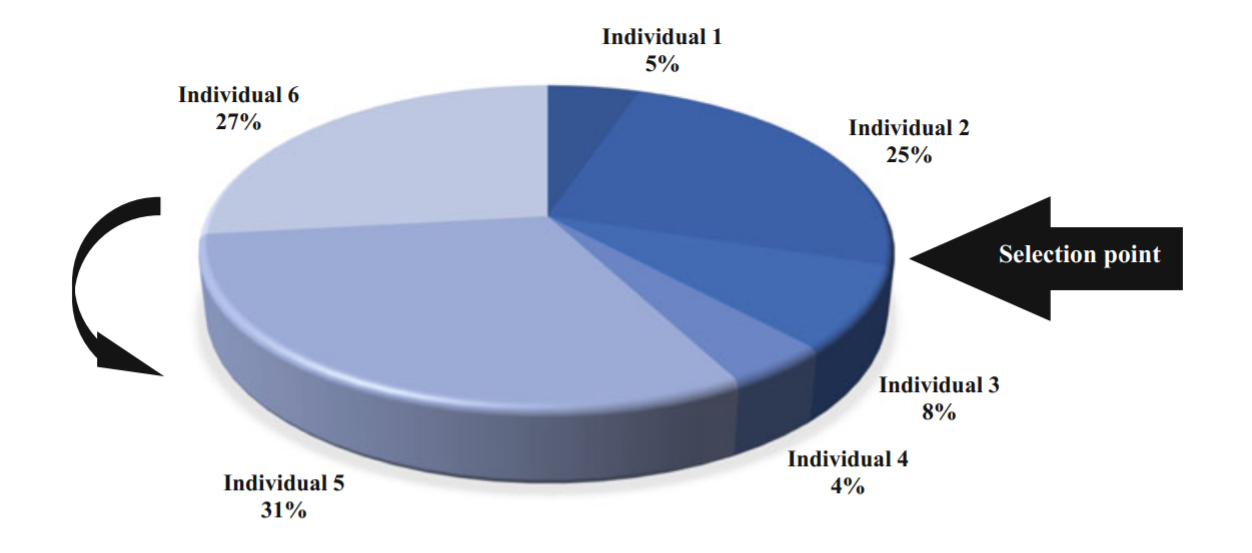
\includegraphics[width=\textwidth]{Img_C2_2.2/FIG_1.png} 
    \caption{Ejemplo mecanismo de la rueda de ruleta en algoritmos geneticos.}
    \label{fig:fig6}
\end{figure}

%Modificar la imagen a español

\begin{table}[h!]
  \centering
  \begin{adjustbox}{width=.75\textwidth}
  \begin{tabular}{|l|l|l|}
\hline
Numero individual & Valor de condición & \% del total \\ \hline
1                 & 12                 & 5            \\ \hline
2                 & 55                 & 24           \\ \hline
3                 & 20                 & 8            \\ \hline
4                 & 10                 & 4            \\ \hline
5                 & 70                 & 30           \\ \hline
6                 & 60                 & 26           \\ \hline
Total             & 227                & 100          \\ \hline
\end{tabular}  
  \end{adjustbox}
  \caption{Detalles de los individuos en la imagen 2.6.}
  \label{table:tab1}
\end{table}

\pagebreak
Se puede ver que el mejor individuo (\#5) tiene la mayor parte de la rueda de la ruleta, mientras que el sujeto (\#4) tiene la menor parte. Este mecanismo simula la selección natural de los individuos mas aptos en la naturaleza. Ya que la ruleta es un operador estocástico, los individuos pobres tienen una menor probabilidad de participar en la creación de la siguiente genereción.
\\

La rueda de la ruleta es unicamente uno de los muchos operadores de selección para algoritmos genéticos.
%citar 10.1007/978-3-319-93025-1_4 
\\

Algunas otras técnicas de selección de operadores son:
\begin{itemize}
\item Selección de Boltzmann
\item Selección de Torneo
\item Selección de Rango
\item Selección Steady state
\item Selección de Truncation 
\item Selección Local
\item Selección Fuzzy
\item Selección Fitness uniform 
\item Selección Proporcional
\item Selección de Rango lineal  
\item Reproducción Steady-state

\end{itemize}


\subsubsection{Técnicas de cruza.}
\subsubsection{Técnicas de mutación.}
\pagebreak
\end{document}
